%% Artigo do TCC II (pesquisa prática) no modelo UNOESC (abnTeX2).
%% Compilar no Overleaf com pdfLaTeX + Biber (Menu > Settings).
\PassOptionsToPackage{english, main = brazilian}{babel}
\PassOptionsToPackage{hyperfootnotes = false}{hyperref}
\documentclass[
  article,
  a4paper,
  12pt,
  fleqn,
  oneside,
  chapter = TITLE,
  section = TITLE,
]{abntex2}

\usepackage[
  BibURLs = true,%% endereço escrito por extenso nas referências (ABNT)
  ABNTNum = none,
]{unoesc-article}

%% Compilação mais rápida (limite de tempo do Overleaf gratuito):
%% sem expansão de fonte do microtype e "²" sem carregar a fonte cm-super
\microtypesetup{expansion=false}
\DeclareUnicodeCharacter{00B2}{\textsuperscript{2}}

%% Citações no padrão (HASTIE; TIBSHIRANI; FRIEDMAN, 2009), sem iniciais extras
\ExecuteBibliographyOptions{uniquename=false, uniquelist=false}

%% Espaço acima e abaixo das equações (o modelo deixa zero)
\AtBeginEnvironment{equation}{\vspace{6pt}}
\AfterEndEnvironment{equation}{\vspace{2pt}}

%% Níveis de título pedidos na estrutura do artigo (UNOESC):
%% 1 MAIÚSCULO NEGRITO; 1.1 MAIÚSCULO ITÁLICO; 1.1.1 minúsculo itálico
\renewcommand*{\ABNTEXsubsectionfont}{\ABNTEXpartfont\itshape}
\renewcommand*{\ABNTEXsubsubsectionfont}{\ABNTEXpartfont\itshape}

\addbibresource{referencias.bib}

%% Mesmo título do TCC I; o subtítulo vai em linha menor, sem maiúsculas, para o título ocupar menos linhas
\titulo{\texorpdfstring{%
  Modelagem preditiva da valorização imobiliária em Chapecó/SC\\[2pt]%
  \NoCaseChange{\large Comparação de algoritmos de aprendizado de máquina}%
}{Modelagem preditiva da valorização imobiliária em Chapecó/SC: comparação de algoritmos de aprendizado de máquina}}

\makeatletter
\let\@fnsymbol\@arabic
\makeatother
\autor{%
  Ana Carla Londero Cazarotto%
  \thanks{%
    \affil{Graduanda em Sistemas de Informação pela UNOESC; Chapecó}%
    \sep\email{ana.cazarotto@unoesc.edu.br}%
  }%
  \and Álvaro Gianni Pagliari%
  \thanks{%
    \affil{Professor orientador do curso de Sistemas de Informação da UNOESC; Chapecó}%
    \sep\email{alvaro.pagliari@unoesc.edu.br}%
  }%
}

\data{}

\begin{document}

\pretextual

\begin{paginadetitulo}

    %% Título nas propriedades do PDF: o modelo usa \thetitle, que traria o "\\" do subtítulo
    \hypersetup{pdftitle={Modelagem preditiva da valorização imobiliária em Chapecó/SC: comparação de algoritmos de aprendizado de máquina}}

    \begin{ambienteresumo}
    Este trabalho investigou se é possível estimar o valor de casas e apartamentos em Chapecó/SC, hoje e ao longo dos anos, com aprendizado de máquina aplicado a anúncios públicos. Foram coletados, por \textit{web scraping}, 46.383 registros de oito imobiliárias locais entre março e agosto de 2026, que resultaram em 3.242 casas e apartamentos válidos após unificação, deduplicação e limpeza. A análise exploratória mostrou preços muito assimétricos, a área e o bairro como principais determinantes e preços anunciados rígidos: 95,9\% não mudaram entre coletas consecutivas. Como cinco meses de anúncios não medem valorização, foi construído um histórico simulado de 2016 a 2025 com um índice que combina a inflação (IPCA) e o custo da construção (INCC), a partir de séries oficiais do Banco Central. Dezoito combinações de algoritmo e alvo foram comparadas com validação cruzada agrupada por imóvel, e o erro foi medido apenas nos preços reais. Os modelos de \textit{boosting} (CatBoost, XGBoost e Gradient Boosting) foram os melhores; o \textit{ensemble} final obteve R² de 0,799 e erro percentual mediano de 14,5\% em apartamentos, e R² de 0,576 e 19,2\% em casas. A valorização estimada foi de +4,33\% ao ano para apartamentos e +4,17\% para casas. Os resultados foram publicados em uma interface web. Conclui-se que a abordagem é viável como apoio à decisão, mas a valorização passada é uma hipótese que precisa ser validada com dados de transações reais.

    \palavraschave{Aprendizado de máquina. Mercado imobiliário. Precificação de imóveis. Valorização imobiliária. \textit{Web scraping}.}
    \end{ambienteresumo}

\end{paginadetitulo}

\textual

%% ===================================================================
\section{INTRODUÇÃO}\label{sec:intro}

Saber quanto vale um imóvel, e quanto ele pode valer daqui a alguns anos, é uma dúvida comum de quem compra, vende ou investe. Em cidades de médio porte como Chapecó, no oeste de Santa Catarina, essa resposta depende quase sempre da experiência de corretores, porque os índices de preços de imóveis existentes cobrem apenas as grandes capitais. Ao mesmo tempo, as imobiliárias da cidade publicam diariamente milhares de anúncios com preço, área, número de quartos e bairro, um volume de dados que pode ser organizado e analisado de forma sistemática.

Diante disso, este trabalho parte de duas questões: é possível construir, a partir de anúncios coletados automaticamente, um modelo que estime o valor de casas e apartamentos em Chapecó com erro aceitável? E, como a coleta cobre poucos meses, de que forma é possível estimar coerentemente quanto esse imóvel valia nos anos anteriores e quanto pode valer nos próximos? Complementarmente, busca-se identificar quais variáveis mais influenciam o preço e qual algoritmo de aprendizado de máquina apresenta o melhor desempenho para os dados disponíveis.

A pesquisa se justifica pela ausência de um indicador de preços para o município, pela relevância econômica do setor imobiliário local e pela possibilidade de oferecer uma ferramenta gratuita e transparente de apoio à decisão. Do ponto de vista acadêmico, o trabalho aplica e compara técnicas de aprendizado de máquina em uma base regional construída do zero, documentando também as limitações encontradas, como a rigidez do preço anunciado.

O objetivo geral é comparar algoritmos de aprendizado de máquina para estimar o valor atual e projetar a valorização de casas e apartamentos em Chapecó/SC. Os objetivos específicos são: coletar e organizar anúncios de imobiliárias locais; realizar a limpeza e a análise exploratória dos dados; treinar e comparar modelos de regressão com métricas adequadas; construir uma estimativa de valorização baseada em índices oficiais; e disponibilizar os resultados em uma interface web.

%% ===================================================================
\section{REVISÃO BIBLIOGRÁFICA}\label{sec:revisao}

\subsection{PRECIFICAÇÃO E VALORIZAÇÃO DE IMÓVEIS}

O preço de um imóvel pode ser entendido como a soma dos valores implícitos de suas características, como área, número de dormitórios e localização. Essa ideia, formalizada pela teoria dos preços hedônicos, sustenta a maior parte dos modelos estatísticos de avaliação imobiliária \cite{rosen1974}. No Brasil, a norma de avaliação de imóveis urbanos admite o uso de modelos de inferência estatística para estimar valores de mercado, desde que se demonstre a qualidade do ajuste aos dados \cite{abnt14653}.

No contexto local, \textcite{reza2025} estudaram os fatores que influenciam o preço de apartamentos anunciados em Chapecó por meio de regressão múltipla com o logaritmo do preço como variável dependente, e concluíram que a área útil, o número de quartos e a disponibilidade de garagem estão entre os principais determinantes. Em revisão das pesquisas publicadas entre 2018 e 2023, \textcite{ferreira2024} identificou o crescimento do uso de redes neurais e de algoritmos supervisionados para prever preços de imóveis, com desempenho frequentemente superior ao dos modelos hedônicos lineares, e apontou a escassez de estudos brasileiros sobre o tema. O mercado de Chapecó, por sua vez, é marcado pelo crescimento urbano e pela expansão da produção imobiliária, característicos de cidades médias \cite{silva2023}.

Para acompanhar a evolução dos preços ao longo do tempo, o Índice FipeZap utiliza anúncios publicados na internet, estratificados por localização e número de dormitórios, mas não contempla Chapecó \cite{fipe2023}. Uma alternativa clássica para medir valorização é comparar o preço do mesmo imóvel em dois momentos, técnica conhecida como vendas repetidas, que elimina as diferenças de tamanho e padrão entre imóveis distintos \cite{bailey1963,case1989}. Essa técnica, entretanto, depende de um histórico longo de preços do mesmo bem, o que não existe quando os dados são coletados por poucos meses.

\subsection{APRENDIZADO DE MÁQUINA PARA REGRESSÃO}

O aprendizado de máquina reúne métodos que permitem a um programa aprender padrões a partir de exemplos, sem que cada regra seja programada explicitamente \cite{russell2021}. A estimativa de preços é um problema de aprendizado supervisionado do tipo regressão, pois o modelo aprende a partir de imóveis com preço conhecido para prever um valor numérico contínuo \cite{james2021}.

Os modelos lineares são o ponto de partida mais simples. A regressão linear múltipla estima um peso para cada variável e é fácil de interpretar, mas supõe que o preço seja uma soma linear das características \cite{hastie2009}. As versões regularizadas Ridge e Lasso acrescentam uma penalidade ao tamanho dos pesos, o que estabiliza o modelo quando as variáveis são correlacionadas entre si, e no caso do Lasso pode zerar variáveis pouco úteis \cite{hoerl1970,tibshirani1996}.

Os modelos baseados em árvores de decisão capturam relações não lineares e interações entre variáveis. O Random Forest treina muitas árvores em amostras aleatórias dos dados e faz a média das previsões, o que o torna robusto a valores atípicos \cite{breiman2001}. O \textit{gradient boosting}, por sua vez, constrói as árvores em sequência, cada uma corrigindo o erro das anteriores \cite{friedman2001}. Duas implementações desse princípio se destacam em dados tabulares: o XGBoost, que acrescenta regularização e amostragem para treinar de forma rápida e estável \cite{chen2016}, e o CatBoost, que trata variáveis categóricas, como o bairro, de forma a reduzir o vazamento de informação do alvo durante o treino \cite{prokhorenkova2018}.

Também foram considerados métodos de outras famílias. As redes neurais do tipo perceptron multicamadas combinam as variáveis em camadas de neurônios e podem representar padrões complexos, mas costumam exigir mais dados e ajuste cuidadoso \cite{geron2019}. A regressão por vetores de suporte busca uma função que passe a uma distância tolerada da maioria dos pontos e é sensível à escala das variáveis e do alvo \cite{drucker1997}. Mais recentemente, o TabPFN propôs um modelo pré-treinado em milhões de tabelas sintéticas, capaz de prever em bases pequenas sem ajuste de parâmetros \cite{hollmann2025}.

\subsection{AVALIAÇÃO DE MODELOS}

Para que o erro medido represente o desempenho em imóveis novos, os dados de teste devem ser separados antes de qualquer decisão de modelagem, e a escolha entre candidatos deve ser feita por validação cruzada dentro do conjunto de treino \cite{kohavi1995}. Quando um mesmo objeto aparece em várias linhas da base, todas as suas linhas precisam ficar do mesmo lado da divisão, caso contrário o modelo é avaliado em exemplos que já viu \cite{hastie2009}.

As métricas usuais em regressão são o erro médio absoluto (MAE), que expressa o erro típico em reais; a raiz do erro quadrático médio (RMSE), que penaliza mais os erros grandes; e o coeficiente de determinação (R²), que indica a fração da variação dos preços explicada pelo modelo \cite{james2021}. O erro percentual absoluto médio (MAPE) é intuitivo, mas torna-se instável quando há valores reais muito pequenos, situação comum em bases com erros de cadastro; nesses casos, o erro percentual mediano é uma alternativa robusta. Para medir a incerteza de uma estimativa, a reamostragem \textit{bootstrap} sorteia repetidamente os dados com reposição e observa a variação do resultado \cite{efron1993}. Já a teoria da credibilidade fornece uma forma de combinar uma estimativa baseada em poucos dados com uma referência mais estável, dando a cada uma um peso proporcional à quantidade de informação disponível \cite{buhlmann2005}.

%% ===================================================================
\section{PROCEDIMENTOS METODOLÓGICOS}\label{sec:metod}

\subsection{TIPO E ABORDAGEM DA PESQUISA}

Quanto à natureza, a pesquisa é aplicada, pois busca resolver um problema prático: estimar o valor de imóveis em um município específico. Quanto à abordagem, é quantitativa, uma vez que se baseia em dados numéricos e em técnicas estatísticas e computacionais. Quanto aos objetivos, é exploratória e descritiva, por investigar um tema pouco estudado no contexto local e descrever os padrões encontrados nos dados \cite{gil2002}. Quanto aos procedimentos, trata-se de pesquisa documental, por usar anúncios publicados na internet e séries oficiais de índices econômicos, e experimental, por comparar modelos sob as mesmas condições controladas \cite{prodanov2013}. O desenvolvimento seguiu as fases do CRISP-DM: entendimento do problema, entendimento dos dados, preparação, modelagem, avaliação e implantação \cite{chapman2000,shearer2000}.

\subsection{INSTRUMENTO DE COLETA DE DADOS}

O instrumento de coleta foi um conjunto de programas em Python que extraem automaticamente os anúncios de venda de oito imobiliárias de Chapecó. Quatro delas tiveram as páginas HTML lidas diretamente e quatro forneceram os dados por meio de interfaces de programação (APIs) usadas pelos próprios sites \cite{mitchell2018}. Foram feitas doze coletas entre 23 de março e 2 de agosto de 2026, cada uma gravada em um banco SQLite datado. Os campos coletados foram preço, bairro, cidade, tipo de imóvel, área total, área privativa, quartos, banheiros, vagas e data da coleta. Nenhuma imobiliária disponibilizou o endereço de forma utilizável, de modo que a localização ficou restrita ao bairro.

Além dos anúncios, foram obtidas as séries mensais oficiais do Índice Nacional de Preços ao Consumidor Amplo (IPCA, série 433) e do Índice Nacional de Custo da Construção (INCC, série 192) no Sistema Gerenciador de Séries Temporais do Banco Central do Brasil \cite{bcbsgs}.

\subsection{TABULAÇÃO DOS DADOS}

As doze coletas somaram 46.383 registros e foram unificadas em uma única base, com uma tabela de imóveis identificados pelo código do anúncio e uma tabela com o histórico de preços de cada imóvel em cada coleta. Grafias diferentes do mesmo bairro foram padronizadas. Como uma mesma casa pode ser anunciada por mais de uma imobiliária, os anúncios foram agrupados por cidade, tipo, área arredondada, quartos, banheiros, vagas e bairro, e cada grupo foi consolidado pela mediana do preço e das áreas. Os tipos de imóvel, escritos livremente pelas imobiliárias, foram mapeados para um catálogo fixo. O processo resultou em 4.266 imóveis únicos, dos quais 3.354 eram casas ou apartamentos e 3.283 tinham preço e área informados. Para a análise exploratória, foram mantidos os 3.242 com preço entre R\$ 50 mil e R\$ 20 milhões e área entre 20 m² e 2.000 m² (Figura~\ref{fig:funil}). Na modelagem, partiu-se dos 3.283, e a remoção dos valores atípicos foi feita dentro do treino, como descrito a seguir. A manipulação foi feita com a biblioteca pandas \cite{mckinney2017}.

\begin{figure}[!htb]
  \caption{Funil de dados, da coleta à base de modelagem}
  \label{fig:funil}
  \centering
  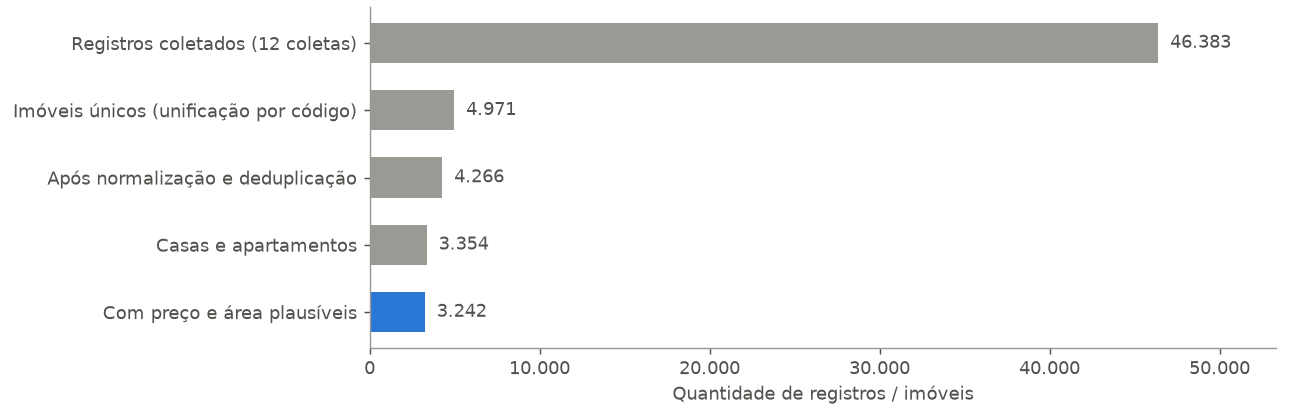
\includegraphics[width=0.85\linewidth]{Figuras/eda_01_funil_dados.png}
  \fonte{Elaborada pela autora (2026).}
\end{figure}

\subsection{TÉCNICA DE ANÁLISE DOS DADOS}

A análise começou pela estatística descritiva e pela análise exploratória \cite{tukey1977}, que orientaram as decisões de modelagem. Em seguida, casas e apartamentos foram modelados separadamente. Para cada tipo, os dados foram divididos por imóvel em 80\% para treino e 20\% para teste, com semente aleatória fixa, antes de qualquer tratamento. As regras de limpeza foram aprendidas somente no treino: bairros com menos de dez imóveis foram agrupados em ``outros'', as variáveis numéricas foram limitadas aos percentis de 2\% e 98\% e os valores atípicos de preço e de preço por m² foram removidos pelo critério do intervalo interquartil (1,5 vez).

Para estimar a valorização ao longo dos anos, foi construído um índice com a média simples das variações mensais do IPCA e do INCC. A lógica é que o terreno e o imóvel como um todo tendem a acompanhar a inflação geral, enquanto a construção tende a acompanhar o custo de construir. Com esse índice, todos os preços reais foram levados ao mês de referência (agosto de 2026) e, para cada imóvel, foram gerados dez registros simulados, um para junho de cada ano entre 2016 e 2025:
\begin{equation}
P_{\text{jun}/Y} = \frac{P_{\text{ref}}}{I_{\text{ref}} / I_{\text{jun}/Y}}
\label{eq:simulacao}
\end{equation}
em que $P_{\text{ref}}$ é o preço no mês de referência e $I$ é o nível do índice. Assim, a base de modelagem passou a ter 3.283 linhas reais (as casas e apartamentos com preço e área informados) e 32.830 simuladas, e o ano foi incluído como variável. Os índices são valores oficiais, mas o passado de cada imóvel é uma hipótese: supõe-se que ele tenha acompanhado o índice.

Foram comparados nove algoritmos (Regressão Linear, Ridge, Lasso, Random Forest, Gradient Boosting, XGBoost, CatBoost, rede neural MLP e SVM), cada um com o alvo em preço e em logaritmo do preço, totalizando 18 candidatos, implementados com scikit-learn \cite{pedregosa2011}, XGBoost e CatBoost. O ranking foi feito por validação cruzada de cinco partes agrupada por imóvel, de modo que o preço real e os simulados de um mesmo imóvel ficassem sempre juntos, e o erro foi medido apenas nas linhas reais. Os três melhores candidatos foram combinados em um \textit{ensemble} com pesos inversamente proporcionais ao erro. A avaliação final usou o conjunto de teste, que não participou de nenhuma escolha, com MAE, RMSE, R² e erro percentual mediano. O MAPE foi descartado porque erros de cadastro, como uma casa anunciada por ``R\$ 1,35'', geram erros de milhões de por cento. O TabPFN foi avaliado em uma etapa anterior do trabalho, mas não foi mantido na comparação final porque cada previsão levava cerca de dois minutos em processador comum e o ganho de precisão não se confirmou no teste.

A projeção do valor futuro combinou duas fontes. A primeira foi a variação do preço anunciado dos mesmos imóveis entre as coletas, por bairro e tipo, com os bairros de poucos dados puxados para a média do tipo pelo peso $n/(n+30)$, em que $n$ é o número de imóveis acompanhados, e com a incerteza estimada por \textit{bootstrap} de 1.000 reamostragens por imóvel. A segunda foi o próprio índice IPCA+INCC. Pela teoria da credibilidade, os anúncios receberam peso $T/(T+12)$, em que $T = 5$ meses de observação, o que resultou em 29\% para os anúncios e 71\% para o índice \cite{buhlmann2005}.

Por fim, os modelos foram publicados em uma interface web desenvolvida com Streamlit \cite{streamlit}. O código-fonte completo, que permite reproduzir todos os resultados, está disponível em repositório público \cite{repositorio}. Ferramentas de inteligência artificial generativa foram utilizadas como apoio à programação e à revisão do código, sob supervisão da autora, que conferiu os resultados apresentados.

%% ===================================================================
\section{ANÁLISE DOS DADOS E RESULTADOS}\label{sec:resultados}

\subsection{ANÁLISE EXPLORATÓRIA}

Apartamentos (45,6\%) e casas (33,0\%) somaram 78,6\% da base normalizada e foram os dois tipos modelados; terrenos e chácaras ficaram de fora, pois seu preço depende principalmente da terra e não da construção. A Tabela~\ref{tab:precos} resume a distribuição dos preços. As casas custam mais no total, mas os apartamentos custam mais por metro quadrado, já que parte da área das casas é terreno.

\begin{table}[!htb]
  \caption{Distribuição de preços de casas e apartamentos}
  \label{tab:precos}
  \centering
  \begin{tabular}{lrr}
    \hline
    & \textbf{Apartamento} & \textbf{Casa} \\
    \hline
    Imóveis & 1.880 & 1.362 \\
    Preço: 10\% mais baratos até & R\$ 320 mil & R\$ 450 mil \\
    Preço mediano & R\$ 690 mil & R\$ 1,00 milhão \\
    Preço: 10\% mais caros a partir de & R\$ 1,50 milhão & R\$ 2,49 milhões \\
    Área mediana & 87 m² & 200 m² \\
    Preço por m² mediano & R\$ 7.423 & R\$ 5.848 \\
    \hline
  \end{tabular}
  \fonte{Elaborada pela autora (2026).}
\end{table}

A distribuição do preço é muito assimétrica, com coeficiente de assimetria de 3,5 em apartamentos e 3,9 em casas; em escala logarítmica, ele cai para 0,3 (Figura~\ref{fig:distribuicao}). Por isso, todos os algoritmos foram testados também com o alvo em logaritmo. A correlação de Spearman com o preço foi de 0,86 para a área em apartamentos e de 0,69 em casas, seguida por vagas (0,69 e 0,48) e quartos (0,66 e 0,54). Esses números confirmam, para um conjunto maior de imóveis, o que \textcite{reza2025} encontraram para apartamentos na cidade, e mostram que a área ordena muito melhor o preço de um apartamento do que o de uma casa. O preço por m² não sobe com o número de quartos, o que indica uma relação não linear entre as variáveis e o preço.

\begin{figure}[!htb]
  \caption{Distribuição dos preços de apartamentos e casas}
  \label{fig:distribuicao}
  \centering
  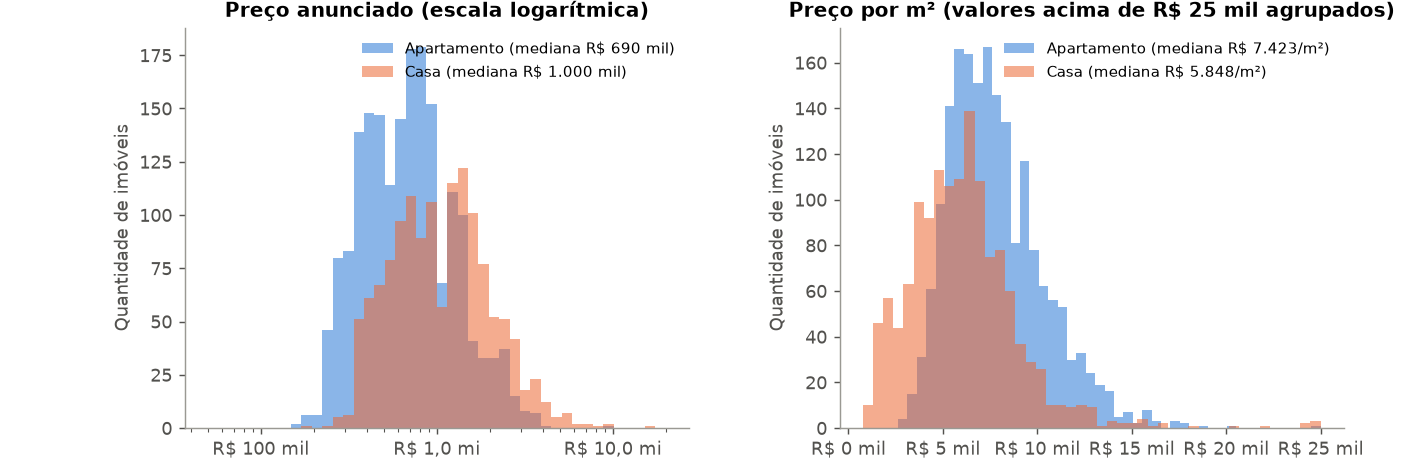
\includegraphics[width=0.85\linewidth]{Figuras/eda_04_distribuicao_precos.png}
  \fonte{Elaborada pela autora (2026).}
\end{figure}

O bairro é a segunda informação mais importante. O preço por m² de apartamentos varia até 70\% entre os bairros listados, com Maria Goretti (R\$ 9.465), Centro (R\$ 8.412), Presidente Médici e Jardim Itália entre os mais caros (Figura~\ref{fig:bairros}). A análise também encontrou erros de cadastro: 19 imóveis com preço abaixo de R\$ 50 mil, como uma casa de 420 m² anunciada por ``R\$ 1,35'', e 89 com área abaixo de 20 m². Nenhuma variável informa o padrão de acabamento, a idade ou o estado de conservação, o que explica parte do erro que permanece nos modelos.

\begin{figure}[!htb]
  \caption{Preço mediano por m² nos principais bairros}
  \label{fig:bairros}
  \centering
  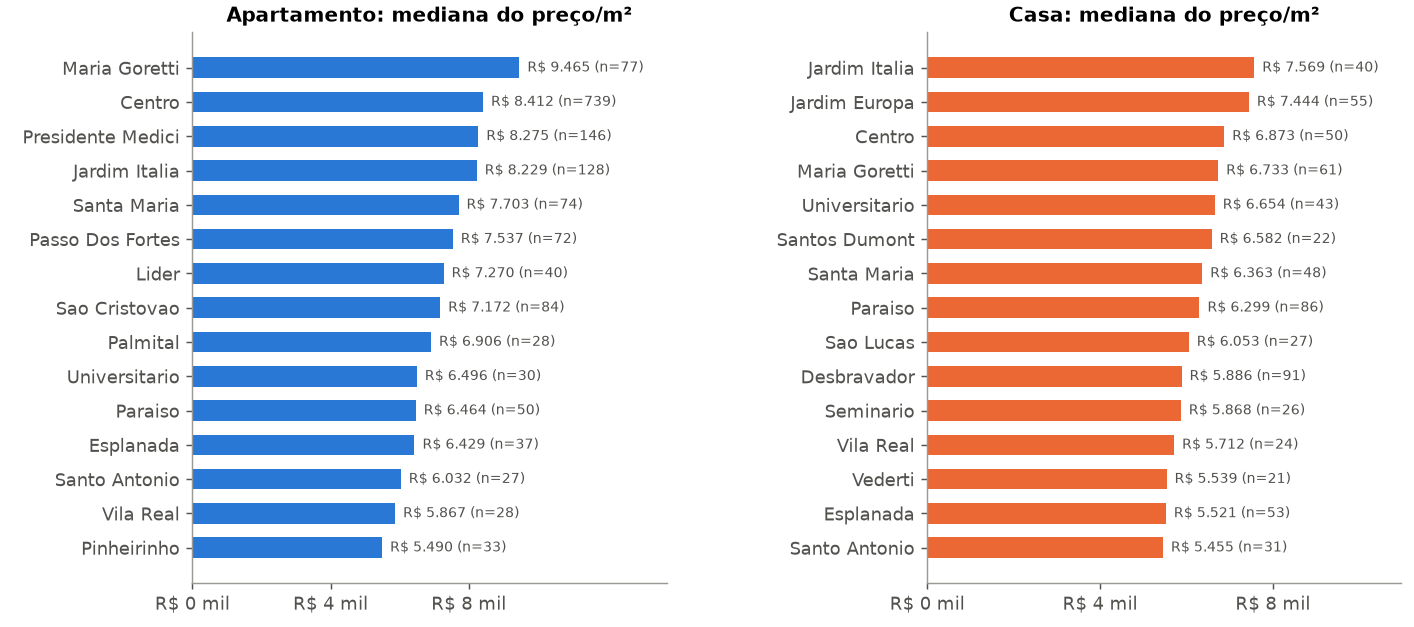
\includegraphics[width=0.85\linewidth]{Figuras/eda_08_preco_m2_bairros.png}
  \fonte{Elaborada pela autora (2026).}
\end{figure}

O comportamento no tempo foi o achado que mais influenciou o trabalho. Comparando o preço do mesmo imóvel entre coletas consecutivas (10.984 comparações), 95,9\% não mudaram, 2,5\% subiram e 1,5\% caíram. Medida apenas pelos anúncios, a valorização foi de +0,89\% ao ano em apartamentos e +0,38\% em casas, muito abaixo da inflação do período. O preço anunciado é definido na entrada do anúncio e raramente reajustado; além disso, os imóveis bem precificados são vendidos e saem da amostra. Um caso real reforçou o problema: um apartamento da cidade comprado por R\$ 160 mil cinco anos antes foi avaliado por um correspondente bancário em cerca de R\$ 235 mil, o que equivale a +7,99\% ao ano. Esse resultado motivou a construção do histórico simulado pelo índice IPCA+INCC.

\subsection{O ÍNDICE IPCA+INCC}

Nos últimos dez anos, o índice combinado variou em média +5,80\% ao ano, entre +3,60\% em 2017 e +11,95\% em 2021 (Figura~\ref{fig:indice}). Nos últimos cinco anos, a média foi de +5,95\% ao ano, contra +5,30\% do IPCA e +6,60\% do INCC isolados. Aplicado ao caso real, o índice levaria o apartamento de R\$ 160 mil a cerca de R\$ 214 mil, um erro de $-9\%$ em relação à avaliação bancária, contra $-29\%$ da medida feita apenas com anúncios. Por se tratar de um único caso, ele foi usado somente como conferência, e não para escolher o índice.

\begin{figure}[!htb]
  \caption{Variação anual do índice IPCA+INCC}
  \label{fig:indice}
  \centering
  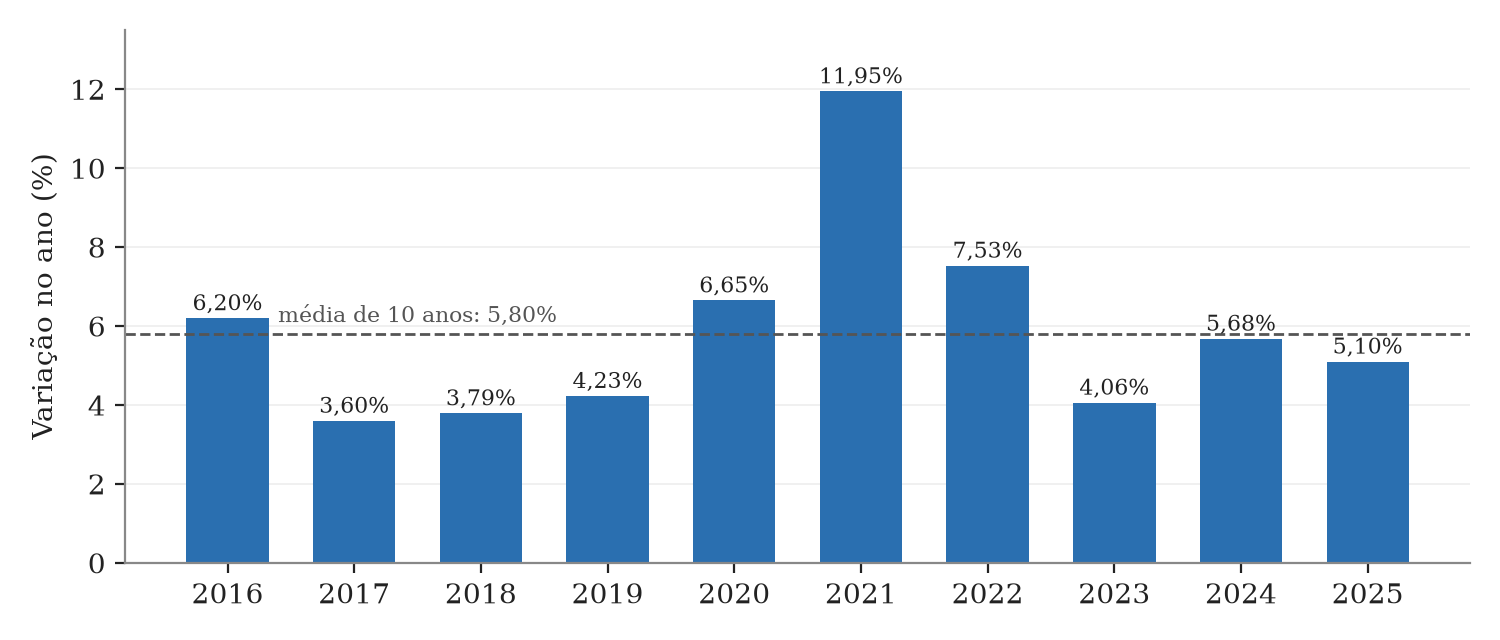
\includegraphics[width=0.85\linewidth]{Figuras/v3_indice_ipca_incc.png}
  \fonte{Elaborada pela autora (2026), com dados do \textcite{bcbsgs}.}
\end{figure}

Antes de adotar o índice, foi testada a hipótese de que a taxa de juros explicaria a valorização. Com 25 anos de dados mensais do Banco Central e três períodos de teste, os modelos com Selic só superaram a média histórica no primeiro período (a partir de 2017); nos dois mais recentes, a média simples de dez anos foi melhor. Por isso, os juros não foram usados na projeção.

\subsection{COMPARAÇÃO DOS MODELOS}

A Figura~\ref{fig:ranking} apresenta os 18 candidatos na ordem da validação cruzada, com o R² obtido no teste, e a Tabela~\ref{tab:modelos} resume os principais. Em apartamentos, o \textit{ensemble} foi formado por CatBoost e XGBoost com alvo em logaritmo e XGBoost com alvo em preço; em casas, por CatBoost, Gradient Boosting e XGBoost, todos com alvo em preço.

\begin{figure}[!htb]
  \caption{R² no teste dos 18 candidatos, na ordem da validação cruzada}
  \label{fig:ranking}
  \centering
  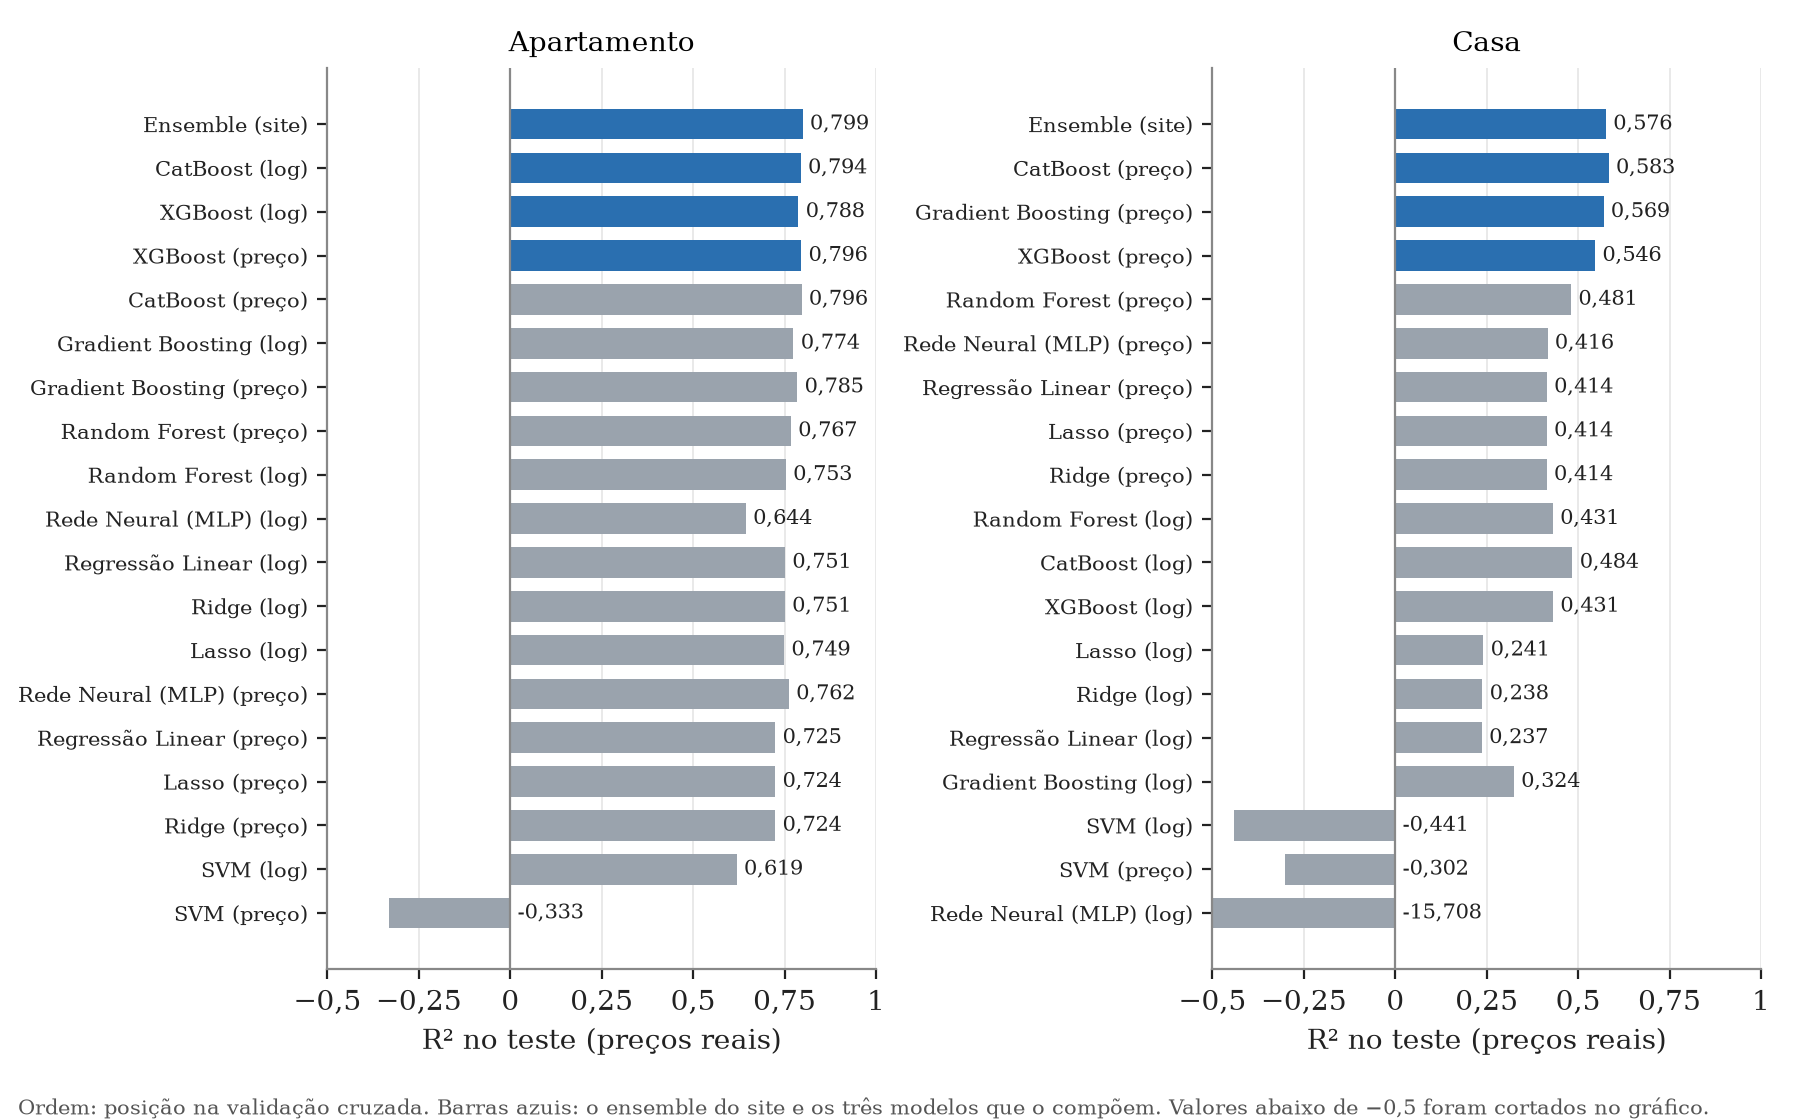
\includegraphics[width=\linewidth]{Figuras/v3_ranking_r2.png}
  \fonte{Elaborada pela autora (2026).}
\end{figure}

\begin{table}[!htb]
  \caption{Desempenho no teste (preços reais) dos principais modelos}
  \label{tab:modelos}
  \centering
  \small
  \begin{tabular}{llrrr}
    \hline
    \textbf{Tipo} & \textbf{Modelo} & \textbf{MAE (R\$)} & \textbf{R²} & \textbf{Erro mediano} \\
    \hline
    Apartamento & \textit{Ensemble} (site) & 121.523 & 0,799 & 14,5\% \\
    & CatBoost (log) & 122.566 & 0,794 & 14,2\% \\
    & Random Forest (preço) & 127.385 & 0,767 & 13,8\% \\
    & Regressão Linear (log) & 132.642 & 0,751 & 15,2\% \\
    & Rede Neural MLP (log) & 145.302 & 0,644 & 16,2\% \\
    & SVM (preço) & 316.157 & $-$0,333 & 39,3\% \\
    \hline
    Casa & \textit{Ensemble} (site) & 296.373 & 0,576 & 19,2\% \\
    & CatBoost (preço) & 295.388 & 0,583 & 19,8\% \\
    & Random Forest (preço) & 322.386 & 0,481 & 19,4\% \\
    & Regressão Linear (preço) & 364.198 & 0,414 & 29,1\% \\
    & Rede Neural MLP (preço) & 360.230 & 0,416 & 27,0\% \\
    & SVM (preço) & 536.631 & $-$0,302 & 43,5\% \\
    \hline
  \end{tabular}
  \fonte{Elaborada pela autora (2026).}
\end{table}

Os modelos de \textit{boosting} foram os melhores nos dois tipos, o que é coerente com a análise exploratória: o preço não é uma soma linear das características, já que o efeito da área muda de um bairro para outro e o preço por m² não cresce com os quartos. O CatBoost liderou a validação cruzada nos dois segmentos, o que se explica pelo tratamento que ele dá a variáveis categóricas como o bairro \cite{prokhorenkova2018}. Os modelos lineares ficaram de 14\% a 22\% piores no MAE da validação, e Ridge e Lasso tiveram praticamente o mesmo resultado da regressão linear, pois as poucas variáveis não causavam instabilidade a ser corrigida. A rede neural e o SVM ficaram entre os piores: com cerca de mil imóveis por tipo, há poucos exemplos para a rede, e o SVM com o alvo em reais obteve R² negativo, ou seja, pior do que prever a média. Em casas, o alvo em logaritmo piorou todos os algoritmos, porque o modelo passa a acertar o valor típico e subestima as casas caras, que concentram o erro em reais.

O \textit{ensemble} final obteve R² de 0,799 em apartamentos e 0,576 em casas, praticamente igual ao de uma versão treinada apenas com os anúncios reais (0,795 e 0,559). Esse empate era esperado, pois o histórico simulado não traz informação nova sobre qual imóvel vale mais; o ganho está em permitir que o modelo responda quanto o imóvel valia em anos anteriores. Na prática, o valor estimado ficou a menos de 20\% do preço anunciado em 66,9\% dos apartamentos e 50,6\% das casas de teste. A Figura~\ref{fig:previsto} mostra que o modelo tende a subestimar os imóveis mais caros, para os quais há menos exemplos na base.

\begin{figure}[!htb]
  \caption{Preço estimado pelo \textit{ensemble} em relação ao preço anunciado (teste)}
  \label{fig:previsto}
  \centering
  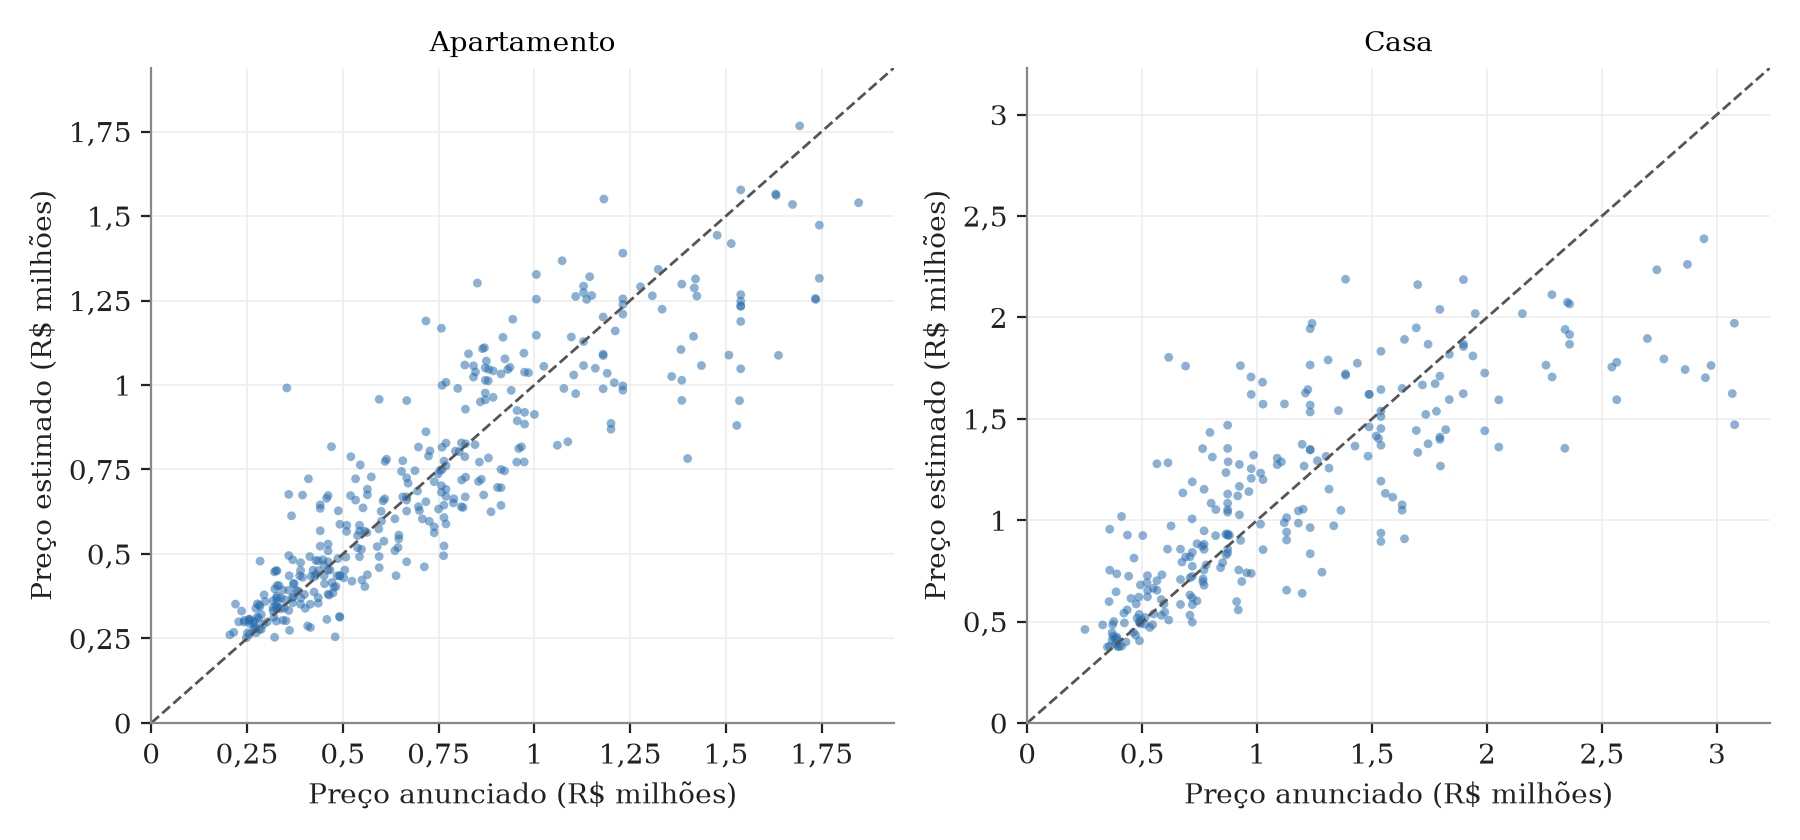
\includegraphics[width=\linewidth]{Figuras/v3_previsto_vs_real.png}
  \fonte{Elaborada pela autora (2026).}
\end{figure}

A diferença entre os tipos também foi coerente com os dados. Casas reúnem imóveis muito diferentes sob o mesmo rótulo, como sobrados, casas geminadas e casas em terrenos grandes, e a área explica menos o seu preço. Quando os anúncios com erros de cadastro foram mantidos no teste, o R² caiu para 0,629 em apartamentos e 0,405 em casas, o que mostra o peso desses erros na base.

\subsection{VALORIZAÇÃO E PROJEÇÃO}

Combinando os anúncios (29\%) e o índice (71\%), a valorização estimada foi de +4,33\% ao ano para apartamentos, com faixa de +2,64\% a +8,32\%, e de +4,17\% ao ano para casas, com faixa de +2,47\% a +8,17\%. A valorização do caso real (+7,99\% ao ano) ficou dentro da faixa estimada para apartamentos, próxima ao cenário otimista. Como coerência interna, o modelo estimou que os imóveis de teste valiam, em junho de 2021, 73,6\% (apartamentos) e 73,7\% (casas) do valor atual, contra 73,5\% indicados pelo índice; essa comparação mostra que o modelo aprendeu o índice, mas não prova que o passado real tenha sido assim.

Como exemplo, um apartamento de 80 m² privativos no Centro, com dois quartos, dois banheiros e uma vaga, foi estimado em cerca de R\$ 658 mil em agosto de 2026. Com a valorização do bairro (+4,26\% ao ano), ele valeria cerca de R\$ 998 mil em dez anos, entre aproximadamente R\$ 843 mil no cenário pessimista e R\$ 1,46 milhão no otimista.

\subsection{INTERFACE WEB}

Os resultados foram disponibilizados em uma interface web pública, acessível em \url{https://scrapping-estates-ayzubn6w4uizag9pbeh5yq.streamlit.app}. Na aba de estimativa, o usuário informa o tipo, o bairro, a área, os quartos, os banheiros e as vagas, e recebe o valor estimado para hoje, a evolução de 2016 até hoje e a projeção para os próximos anos nos três cenários, além de avisos quando os dados informados estão fora do padrão da base. As demais abas mostram a valorização por bairro, a explicação de cada um dos 18 modelos com o motivo do seu resultado e o conjunto de dados utilizado, com os imóveis reais e o histórico simulado. Em relação aos protótipos planejados no TCC I, o painel com os coeficientes de cada variável foi substituído pela explicação dos modelos, já que os modelos de \textit{boosting} não possuem coeficientes diretamente interpretáveis.

%% ===================================================================
\section{CONCLUSÃO}\label{sec:concl}

Este trabalho mostrou que é possível estimar o valor de casas e apartamentos em Chapecó a partir de anúncios coletados automaticamente, com erro típico de cerca de 15\% para apartamentos e 20\% para casas. Respondendo às questões de pesquisa, o desempenho foi aceitável para apartamentos e moderado para casas; a área e o bairro foram as variáveis mais influentes, seguidas de vagas e quartos; e os algoritmos de \textit{boosting}, em especial o CatBoost, apresentaram o melhor desempenho, enquanto a rede neural e o SVM ficaram entre os piores para o volume de dados disponível.

O principal aprendizado foi que poucos meses de anúncios não medem valorização, porque o preço anunciado quase não muda. A solução adotada, simular o passado de cada imóvel com um índice formado por inflação e custo de construção, deu à projeção uma lógica econômica clara e fez a valorização estimada se aproximar do único caso real disponível. Ainda assim, o passado simulado é uma hipótese, e não um preço observado, e assim deve ser apresentado.

Entre as limitações, destacam-se o uso do preço anunciado no lugar do preço de venda, a falta de endereço, idade e padrão construtivo dos imóveis, o número reduzido de imóveis de alto padrão e a validação da valorização com um único caso real. Como trabalhos futuros, sugere-se obter dados de transações efetivas, como o Imposto sobre Transmissão de Bens Imóveis (ITBI) junto à Prefeitura, para validar o histórico simulado; reunir mais casos reais de compra e avaliação; manter a coleta por mais tempo para medir a valorização diretamente; e incluir informações sobre a idade e o padrão dos imóveis, por exemplo, a partir das fotos dos anúncios.

Por fim, a interface web publicada permite que qualquer pessoa consulte as estimativas e entenda como elas foram produzidas, o que cumpre o propósito de oferecer uma ferramenta transparente de apoio à decisão no mercado imobiliário local.

%% ===================================================================
\postextual
\printbibliography

\end{document}
